\chapter{代数}
又回到最初的起点,呆呆地站在括号前\\
\makebox{}\hfill Adapted from 胡夏

\section*{学习目标}
\begin{todolist}
 \item 理解绝对值的含义,并绘制带有绝对值的函数图像
 \item 解决含有绝对值的方程或者不等式
 \item 计算多项式的除法(被除多项式不超过4次,除式为线性或者二次表达式),并能够识别商和余数
 \item 理解并运用多项式的余数理论和因式理论
 \item 分式表达式的化简运算
 \item 二项展开式$(1+x)^n$在$n$为负数或分数的情况下的运用
\end{todolist}
\clearpage

\section{绝对值}
一个数的\gls{abs},也被称之为modulus。符号为$|x|$,其含义是代表该数字到原点的距离。
如下图所示:
\begin{figure}[H]
\centering
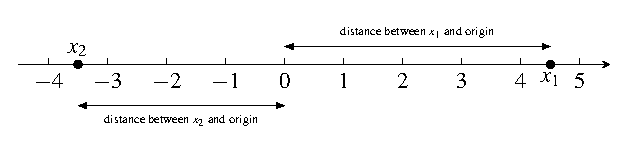
\includegraphics[width=0.8\textwidth]{numbeline}
\caption{数轴以及数轴上的数字}
\end{figure}

\subsection*{绝对值的非负性}
由于绝对值的含义是代表一个长度,因此对任何数字取绝对值都必定大于或者等于$0$。因此,一个正数的绝对值必定是其自身;一个负数的的绝对值是其相反数。$0$的绝对值还是$0$,即可以认为是自身,也可以认为是其相反数。

\subsection*{含有绝对值的运算法则}
常规运算中加入绝对值,要确保最终结果的非负性。因此有如下的运算法则:

\[
\begin{matrix}
|a\times b| = |a| \times |b|  & \left|\frac{a}{b}\right| = \frac{|a|}{|b|}\\
|x^2| =|x|^2 =(-x)^2=x^2 & \sqrt{x^2} =|x|
\end{matrix}
\]

\subsection*{分类讨论的思想求算含有绝对值的方程}
由于一对相反数的绝对值都是同一个数字,因此在解决含有绝对的方程的时候,需要进行分类讨论。

\begin{ExampleBox}
 solve $\left(|x-3|\right)^2-|x-3|-6=0$
 \tcblower
 首先把$|x-3|$作为一个整体,$y$,方程可以改写为:
 \[
 	y^2-y-6=0
 \]
 因此采用因式分解的方式可以得到$(y-3)(y+2)=0$,所以$|x-3|=3$或者$|x-3|=-2$但是很明显不可能任何绝对值是负数,所以只能$|x-3|=3$。
 最后,进行分类讨论
 $x-3$如果是正数,那么$x-3=3$;如果$x-3$是负数,那么$x-3=-3$
 因此最后的结果为$x=6$ or $x=0$
\end{ExampleBox}

\subsection*{含有绝对值的不等式}
对于含有绝对值的不等式,所需要的处理仅仅是把分类讨论的结果改写为不等式即可。但是要结合多项式的意义,明确一下范围。
\begin{ExampleBox}
 solve $|x+3|>5$
 \tcblower
 如果是含有绝对值的方程$|x+3|=5$,那么很简单的分类讨论就结束$x=-8$ 或者 $x=2$。但是现在是不等式,需要结合一下绝对值的意义。\\
 $x+3$作为一个整体,绝对值小于$5$,意味着如果这个整体是正数,不能比$5$更大;如果是负数,不能比$-5$更小。因此实际上就可以等价地写成$-5<x+3<5$进行求解即可,因此最终结果为$-8<x<2$。在两根之内。\\

 第二种理解方案会更快,结合数轴图像$|x+3|=|x-(-3)|$代表$x$与$-3$这个两个数值点的距离。因此$-3$右移$5$和左移$5$分别得到$-8$与$2$。由于该距离小于5,因此在两个数值之间
 \begin{figure}[H]
 \centering
 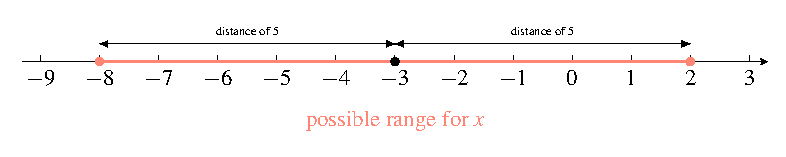
\includegraphics[width=0.8\textwidth]{absineq}
 \caption{$|x+3|$也可以当做是$x$和$-3$之间的距离}
 \end{figure} 
\end{ExampleBox}


\begin{TaskBox}
Find the set of values of $x$ satisfying the inequality $2|2x-a|<|x+3a|$, where $a$ is a positive constant.\\
\makebox{}\hfill Adapted From $2018$ winter qp $31$ $Q1$
\end{TaskBox}

\subsection*{含有绝对值的线性函数图像}
对于$y=|mx+b|$或者$f(x)=|mx+b|$这样的含有绝对值的线性函数,当$y$值大于等于0的时候,绝对值就是自身,因此函数图像没有任何变化;只需要考虑当$y$值小于0的时候,需要取相反数,也就是$y=-[mx+b]$。结合\ref{subsec:Reflection}的内容便知,需要把低于$x$轴下方的图像绕着$x$轴翻折一下。
\begin{figure}[H]
\centering
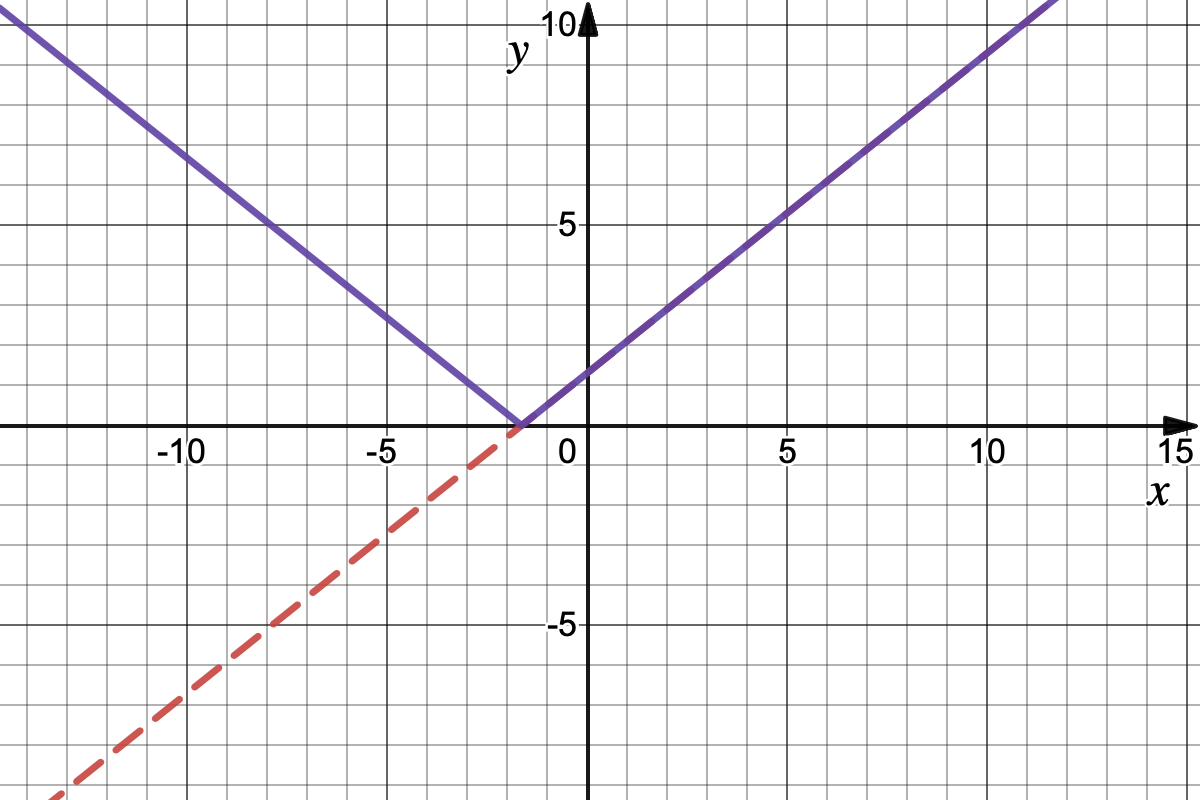
\includegraphics[width=0.8\textwidth]{abs.png}
\caption{红色的虚线图像为普通线性函数,紫色的则是加了绝对值的线性函数}
\end{figure}

点击该\href{https://www.desmos.com/calculator/qkkzxj8wwr}{链接}尝试改变斜率和截距。观察图像变化

\begin{TaskBox}
尽管P3中不考察曲线图像的绝对值化,但还是尝试绘制一下$y=|x^2-5x+6|$的图像,说明其和$y=x^2-5x+6$的关联。加深自己对绝对值的理解
\end{TaskBox}
\clearpage

\section{多项式的运算}
多项式是代数的一颗瑰宝,一座高峰。

\subsection*{多项式的长除法}
形如$a_1x^n+a_2x^{n-1}+\cdots+a_nx+a_{n+1}$的表达式称之为\gls{polynomial}
在小学阶段所学习的竖式除法依旧可以用于多项式当中,称之为长除法。基本思路是将消去最高次项,直至到最后一项

\begin{ExampleBox}
Divide $4x^3-7x-1$ by $2x+1$
\tcblower
先列出长除的表达式:\\
\polylongdiv[stage=1,style=A]{4x^3-7x-1}{2x+1}\\
然后为了消去最高次项$4x^3$,除数$2x+1$必须和$2x^2$相乘:\\
\polylongdiv[stage=3,style=A]{4x^3-7x-1}{2x+1}\\
两项$0x^3$和$2x^3$相减得到$-2x^3$继续重复相消的过程\\
\polylongdiv[stage=9,style=A]{4x^3-7x-1}{2x+1}\\
最后到到常数(零次)项$-1$和$-3$相减得到$+2$。由于已经低于除数的次数(一次),因此长除法结束\\
\polylongdiv[stage=10,style=A]{4x^3-7x-1}{2x+1}\\

最后得到如下的结果:
\[
\fbox{$\frac{4x^3-7x-1}{2x+1}=(2x^2-x-3)+\frac{2}{2x+1}$}
\]
或者说
\[
	(4x^3-7x-1)= (2x^2-x-3)\cdot (2x+1) +2
\]
\end{ExampleBox}

\begin{TaskBox}
 利用长除法,重复计算一下 $4x^3-7x-1$除以$2x^2-x-3$得到的结果,陈述商和余数分别是什么。
\end{TaskBox}

\subsection*{余数理论}
在刚才的例子当中
\[
	\fbox{$4x^3-7x-1$}=\fbox{$2x+1$}\cdot\fbox{$2x^2-x+3$}+\fbox{$2$}
\]
本质上就是为了表达如下的关系:
\[
	\text{Dividend} = \text{Divisor} \cdot \text{Quotient}+\text{Remainder}
\]
这个关系对于任意的$x$都是成立的。因此当我选择特定的$x$的值的时候,比如在这里$x=-\frac{1}{2}$,看看发生了什么事情:
\[
	4\times \left(-\frac{1}{2}\right)^3-7\times\left(-\frac{1}{2} \right)-1 = \left(2\times -\frac{1}{2}+1\right)\cdot \text{Quotient} + \text{Remainder}
\]
所以无需经过复杂的长除,也无需求算Quotient的表达式,我们就能简单优雅的推导出:Remainder $= 2$这样的结论。

\begin{figure}[H]
\centering

\includegraphics[width=0.3\textwidth]{youya.jpeg}
\end{figure}
高不高级,速度不速度?

这就是多项式中非常重要的\gls{remaindertheo}。
\begin{theorem}[Remainder Thoerem]
When a polynomial $f(x)$ is divided by $(x-a)$, the remainder is always $f(a)$\\

When a polynomial $f(x)$ is divided by $(ax-b)$, the remainder is always $f\left(\frac{b}{a}\right)$
\end{theorem}

\subsection*{因式定理}
当多项式可以被另外一个低次表达式除尽的时候的时候,也就是形成了
\begin{center}
Dividend = Divisor $\cdot$ Quotient 
\end{center}
而没有余数,或者称余数为$0$的时候,Divisor就可以改口叫做Factor。因此\gls{factortheo}就是余数定理的特例情况,是当余数为$0$的时候。

\begin{theorem}[Factor Thoerem]
For a polynomial $f(x)$, if $f(a)=0$ then the remainder when when $f(x)$ is divided by $(x-a)$ is zero, making it a factor of the polynomial $f(x)$
\end{theorem}

\begin{TaskBox}
The polynomial $x^3-ax^2+2x+8$, where $a$ is a constant, is denoted by $p(x)$. It is given that $(x-a)$ is a factor of $p(x)$, determine the value of $a$ and factorize the polynomial completely.
\end{TaskBox}
\clearpage


\section{有理分式}
两个多项式相除的结果作为一个表达式,被我们称之为有理分式。比如 $\frac{11x^2+8x+10}{(4x+1)(x^2+3)}$ 尽管下方并没有完全打开括号,分母也必定是一个三次的多项式。并且这种分母的形式表明是两个分式的common denominator。

\subsection*{分式分解}
\gls{partialfrac}是考试当中必考的内容。分母是两个表达式之积,因此上面的有理分式可以化简为两个分式之和。
因此必定可以找到特定的系数$A$,$B$,$C$,能够使得:
\[
	\frac{11x^2+6x+10}{(4x+1)(x^2+3)}=\frac{A}{4x+1}+\frac{Bx+C}{x^2+3}
\]
始终成立。这样,一个分母为三次的多项式就降低为两个低次的有理式之和形式。使得后续的计算更为简单。不过需要记住的是,低次的有理分式之后也得确保分子比分母少一次;因此在第二项的时候不能写$\frac{B}{x^2+3}$
\begin{ExampleBox}
确定上方系数$A$,$B$,$C$
\tcblower
通分之后,确保分子一致即可:
\[A\cdot (x^2+3)+(Bx+C)\cdot (4x+1) \equiv 11x^2+6x+10\]
可以采用列方程组或者带入特定$x$值进行求解。
下略,最后结果为$A=3 \ B=2 \ C=1$
\end{ExampleBox}


考试当中的Partial Fraction一般会有如下的三种形式:牢记拆分能够帮助自己快速解决
\begin{SummBox}
 \begin{itemize}
 	\item 分母当中包含线性因式:\\$\frac{\ldots}{(ax+b)(\ldots)}=\frac{A}{ax+b}+\frac{\ldots}{\ldots}$
 	\item 分母当中包含线性因式的二次方:\\$\frac{\ldots}{(ax+b)^2(\ldots)}=\frac{A}{ax+b}+\frac{B}{(ax+b)^2}+\frac{\ldots}{\ldots}$
 	\item 分母当中包含二次因式:\\$\frac{\ldots}{(ax^2+bx+c)(\ldots)}=\frac{Ax+B}{ax^2+bx+c}+\frac{\ldots}{\ldots}$
 \end{itemize}
\end{SummBox}
\clearpage

\section{二项展开式在非正整数次幂的运用}
一切都要从二项展开式说起,牢记这个公式:
\[
	(a+b)^n={n\choose 0}a^n+{n\choose 1}a^{n-1}b^1+\cdots+{n\choose n-1}a^1b^{n-1}+{n\choose n}b^n
\]

可是,当$n$不是一个正整数的时候,比如$\sqrt{1+x}=(1+x)^{\frac{1}{2}}$甚至是负数的时候,比如$(1+x)^{-2}$,这个关系还能利用吗,想要利用的话需要解决 1)应该写多少项;2)负数和分数的组合数求算 这两个问题
\subsection*{非正整数的次幂}
如果$n$为正整数,那么二项展开式是有限的,共有$n+1$项。但是当$n$不满足这个条件的时候,这个基本框架还能能用的,但是此时已经要变成无穷多项。也就是变成一个无穷\gls{series}:
\begin{align*}
	(1+x)^\frac{1}{2} &=1+{\frac{1}{2}\choose 1}x^1+{\frac{1}{2}\choose 2}x^2+\ldots\\
	(1+x)^{-2} &=1+{-2\choose 1}x^1+{-2\choose 2}x^2+\ldots
\end{align*}

\subsection*{分数和负数的组合数}
在明确了这个之后,接下来要做的事情就是这些组合数的求算 ${\frac{1}{2} \choose 1}$ 和 ${-2 \choose 1}$等,尽管这些组合数不再有任何概率统计上的意义。但还是能依照组合数的定义求算出具体的数值的。
回顾一下正数的情况:${6\choose 4} = \frac{6\times 5\times 4\times 3}{4\times 3\times 2\times 1}$。分式的下方就是正整数$4$的阶乘;而分子上则是从$6$开始连续降$1$,并且确保依旧有$4$个数字;

所以,即使当${n\choose m}$当中$n$不是正整数的时候,依旧可以改写成
\[
	{n\choose m} = \frac{n\times {(n-1)}\times (n-2)\times \ldots \times (n+1-m)}{m\times {(m-1)}\times (m-2)\times \ldots \times1\qquad \qquad} %qquad 用来保持对齐的
\]

\begin{TaskBox}
求算${-2 \choose 2}$,${\frac{1}{2} \choose 3}$等结果
\end{TaskBox}

因此最后,二项展开式可以用于任何次幂的展开。比如:
\begin{align*}
(1+x)^\frac{1}{2} &=1+\frac{1}{2}x^1-\frac{1}{8}x^2+\frac{1}{16}x^3+\ldots\\
(1+x)^{-2} &=1+(-2)x^1+3x^2-4x^3+\ldots
\end{align*}


\subsection*{其他考量}
到此为止,这种展开的基本思路就是这样。但是还有几点值得研究一下。
\subsubsection*{$(1+bx)^n$的展开}
经过我们苦心孤诣地推导,我们得到了:
\[
	(1+\fbox{$x$})^n = 1+\frac{n}{1}\fbox{$x$}^1+\frac{n\times (n-1)}{2\times 1}\fbox{$x$}^2+\frac{n\times (n-1)\times (n-2)}{3\times2\times 1}\fbox{$x$}^3+\ldots
\]
那么,处理$(1+bx)^n$的时候,是不是只需要把\fbox{$bx$}作为一个整体就可以了。因此
\[
	(1+\fbox{$bx$})^n = 1+\frac{n}{1}\fbox{$bx$}^1+\frac{n\times (n-1)}{2\times 1}\fbox{$bx$}^2+\frac{n\times (n-1)\times (n-2)}{3\times2\times 1}\fbox{$bx$}^3+\ldots
\]

\subsubsection*{$(a+x)^n$的展开}
利用$(a+x)^n=a^n\cdot (1+\frac{x}{a})^n$。之后再进行展开:
\[
	a^n(1+\fbox{$\frac{x}{a}$})^n =a^n\left( 1+\frac{n}{1}\fbox{$\frac{x}{a}$}^1+\frac{n\times (n-1)}{2\times 1}\fbox{$\frac{x}{a}$}^2+\frac{n\times (n-1)\times (n-2)}{3\times2\times 1}\fbox{$\frac{x}{a}$}^3+\ldots\right)
\]

\subsubsection*{适用范围}
如果$(1+x)^{-2} =1-2x^1+3x^2-4x^3+\ldots$,
那么我们将这两个多项式函数输入到绘图软件中,会得到这样的结果:
\begin{figure}[H]
\centering
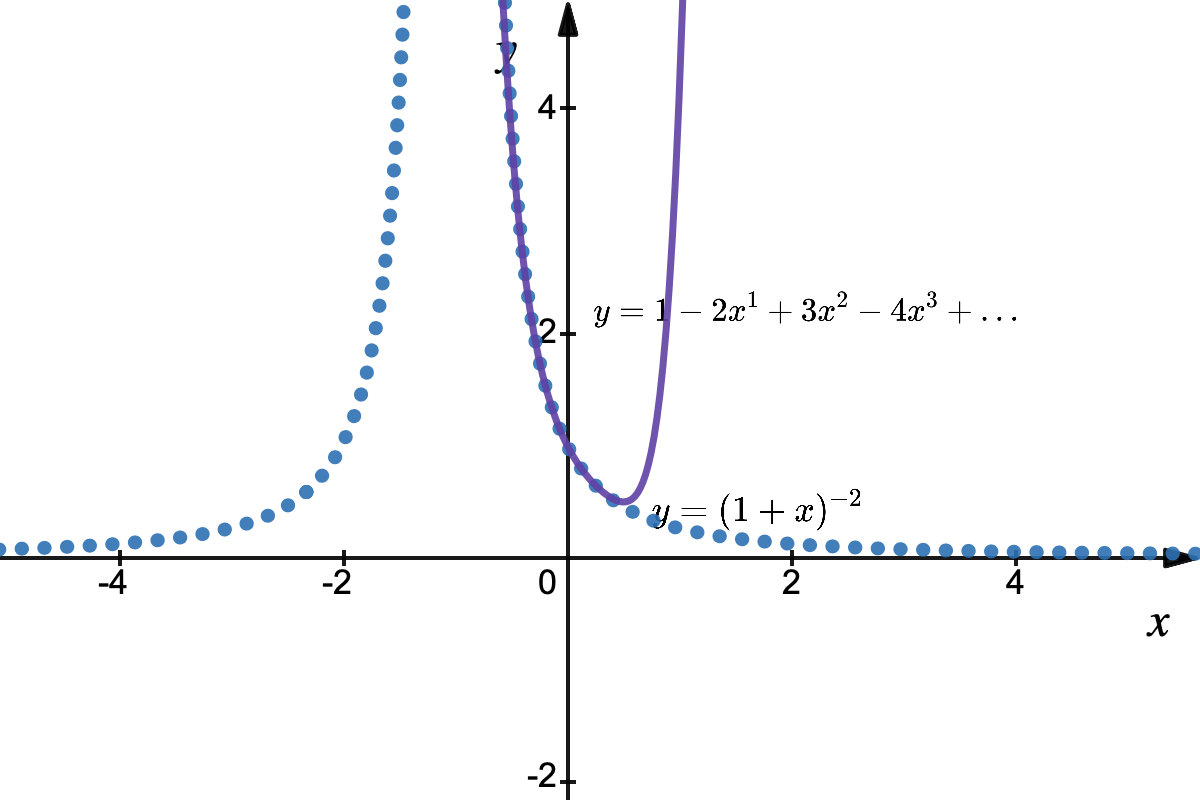
\includegraphics[width=0.8\textwidth]{expand}
\caption{二项展开图像和展开前的一致}
\end{figure}

\begin{TaskBox}
确定哪一个图像是$y=(1+x)^{-2}$的函数图像,哪一个是展开式多项式的图像
\end{TaskBox}

不难发现,展开式和原来的表达式确实很接近,可以点击该\href{https://www.desmos.com/calculator/huhb3kfnjz}{desmos}展开更多项查看。

但是还有一个问题,是展开式的图像仅针对特定的$x$范围是一致的。这个范围是$-1<x<1$或者说$|x|<1$。证明过程不做推导。感兴趣可以点击\href{https://tutorial.math.lamar.edu/classes/calcii/RatioTest.aspx}{Ratio Test}了解更多。

\begin{SummBox}
$(1+x)^n=1+\frac{n}{1}x^1+\frac{n\times(n-1)}{2!}x^2+\frac{n\times(n-1)\times(n-2)}{3!}x^n+\ldots$        when $|x|<1$
\end{SummBox}

这就是非常著名的牛顿广义二项式定理。
